\subsection{Neyman-Pearson Lemma}

\subsubsection{Type I \& Type II errors}
\textbf{Overview} : In a hypothesis test, we are interested in testing a given null hypothesis $H_0$ against some alternative hypothesis $H_1$. Hence, we define some rejection region $\mathcal{R}\subset\mathbb{R}$ such that:
\begin{align*}
    x \in \mathcal{R} \implies \text{reject } H_0 
\end{align*}

\noindent Equivalently, denote that $\overline{\mathcal{R}}$ is the acceptance region. We define the following conditional probability densities:
\begin{itemize}
    \item $f_1(x)$ : Density given that $H_1$ is true.
    \item $f_0(x)$ : Density given that $H_0$ is true.
\end{itemize}

\begin{definition}[Type I \& Type II errors]
    In hypothesis testing, we define the type I error as the probability that we falsely reject the null hypothesis given that the null hypothesis is true. On the other hands, type II error is the probability that we falsely accept the null hypothesis given that the hypothesis is not true:
    \begin{align*}
        \alpha &= P_{H_0}(\mathcal{R}) = \int_\mathcal{R} f_0(x)dx 
        \\ 
        \beta &= P_{H_1}(\overline{\mathcal{R}}) = 1 - \int_\mathcal{R} f_1(x)dx
    \end{align*}
\end{definition}

\noindent There is a trade-off between type I and type II errors as illustrated in the figure below:
\begin{figure}[ht]
    \centering
    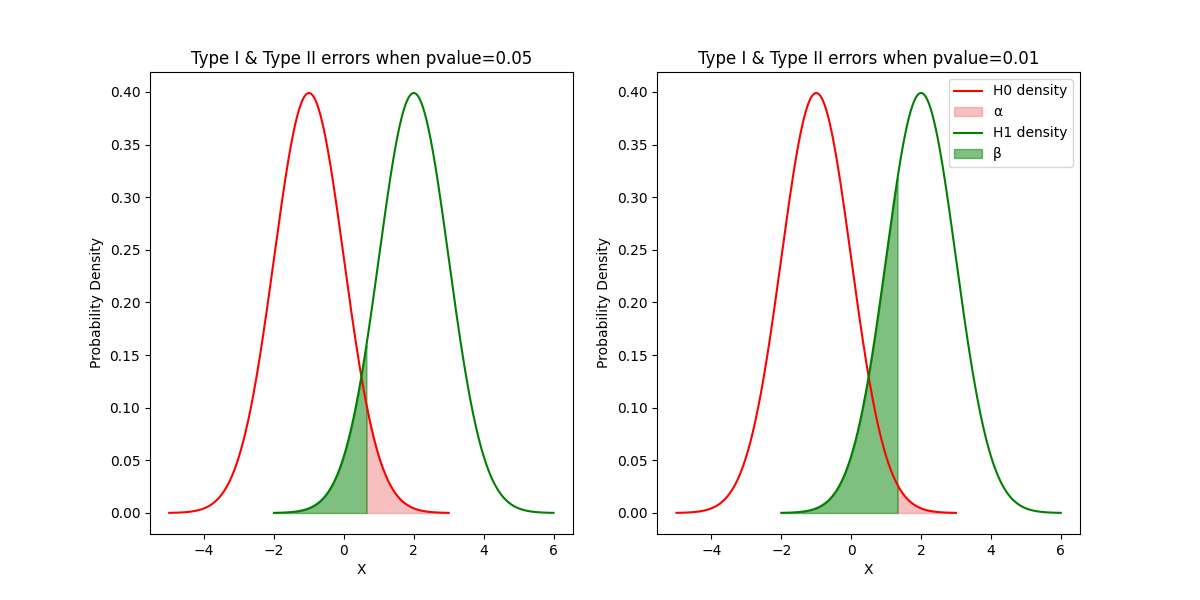
\includegraphics[width=\textwidth]{figures/typeI_typeII_errors_tradeoff.png}
    \caption{Trade-off between type I and type II errors}
    \label{fig:type_I_type_II_errors_tradeoff}
\end{figure}

\begin{definition}[Power of hypothesis test]
    Given a hypothesis test used to test a null hypothesis $H_0$ against an alternative hypothesis $H_1$. The probability:
    \begin{align*}
        P_{H_1}(\mathcal{R}) = \int_{\mathcal{R}} f_1(x)dx = 1 - \beta
    \end{align*}

    \noindent Which denotes the probability that we correctly reject the null hypothesis given that $H_1$ is true  is called the \textbf{Power} of the hypothesis test. Later on we will see that using \textbf{Neyman-Pearson Lemma}, we can prove any hypothesis test has the power of at most the likelihood ratio test's power. 
\end{definition}


\subsubsection{Neyman-Pearson Lemma}
\textbf{Overview} : The Neyman-Pearson Lemma is concerned with maximizing the power of hypothesis test subjected to a certain degree of type I error. Formally, we are trying to solve the following constrained optimization problem:
\begin{align*}
    \text{maximize} &: P_{H_1}(\mathcal{R}) = \int_\mathcal{R} f_1(x)dx 
    \\
    \text{subjected to} &: P_{H_0}(\mathcal{R}) = \int_\mathcal{R}f_0(x) dx \le \alpha
\end{align*}

\begin{theorem}{Neyman-Pearson Lemma}{neyman_pearson_lemma}
    Let $H_0$ and $H_1$ be simple hypotheses. For a constant $c>0$, suppose the likelihood ratio test rejects $H_0$ when $L(X) > c$ has significance level $\alpha\in(0,1)$. \textbf{Then for any other test of $H_0$ with significance level of at most $\alpha$, its power against $H_1$ is at most the power of the likelihood ratio test.}

    \begin{align*}
        \mathcal{R} = \biggCurl{
            x \in \mathbb{R} : L(x) = \frac{f_1(x)}{f_0(x)} > c
        }
    \end{align*}
\end{theorem}

\begin{proof*}[Theorem \ref{thm:neyman_pearson_lemma}]
    Note that the rejection region $\mathcal{R} = \biggCurl{ x \in \mathbb{R} : L(x) = \frac{f_1(x)}{f_0(x)} > c }$ maximizes the quantity:
    \begin{align*}
        \int_{\mathcal{R}} (f_1(x) - cf_0(x))dx
    \end{align*}

    \noindent Because $f_1(x) - cf_0(x) < 0$ for all $x\notin\mathcal{R}$. Therefore, for any other test with rejection region $\mathcal{R}'$ with significance level of at most $\alpha$, we have:
    \begin{align*}
        \int_{\mathcal{R}} (f_1(x) - cf_0(x))dx 
            &\ge \int_{\mathcal{R}'} (f_1(x) - cf_0(x))dx \\
        \implies
        P_{H_1}(\mathcal{R}) - P_{H_1}(\mathcal{R}') 
            &\ge 
            c \biggRound{
                \int_{\mathcal{R}} f_0(x)dx -  \int_{\mathcal{R}'} f_0(x)dx
            } \\
            &= c \biggRound{
                \alpha -  \int_{\mathcal{R}'} f_0(x)dx
            } \\
    \end{align*} 

    \noindent Since $\int_{\mathcal{R}'} f_0(x)dx \le \alpha$, we have:
    \begin{align*}
        P_{H_1}(\mathcal{R}) - P_{H_1}(\mathcal{R}') 
            &\ge 0 \implies P_{H_1}(\mathcal{R}') \le P_{H_1}(\mathcal{R})
    \end{align*} 

    \noindent Hence, for any test with significance level of at most $\alpha$, the power is at most the power of the likelihood ratio test $P_{H_1}(\mathcal{R})$.
\end{proof*}


